\section{Capítulo V - Análisis de resultados}

Este capítulo presenta el análisis de los resultados obtenidos con el sistema propuesto, denominado Controla, cuyo título es: Desarrollo de una aplicación web para el control de cheques, caja chica, viáticos y alertas de pagos a proveedores en una distribuidora farmacéutica utilizando Angular, Python y PostgreSQL. El análisis compara la situación anterior con la situación posterior a la incorporación de las funcionalidades documentadas en los capítulos III y IV.

La comparación no se limita a indicar si el sistema funciona. Se examinan los cambios observados en el tiempo de proceso, la tasa de errores, el personal involucrado y el consumo de insumos. También se interpretan los nuevos flujos de trabajo y se relacionan los resultados con la hipótesis de investigación.

\subsection{Metodología de comparación}

El objetivo de esta comparación fue identificar los cambios producidos en los módulos de Proveedores, Viáticos y Nomenclatura contable. Para cada módulo se analizaron cuatro indicadores: tiempo de proceso, tasa de errores, personal involucrado e insumos consumidos por semana.

El tiempo de proceso (TP) representa el tiempo promedio requerido para completar la operación principal del módulo. La tasa de errores (TE) representa la proporción de incidencias observadas durante la ejecución del proceso. El indicador Personal corresponde al promedio de personas que participan directamente en la operación. El indicador Insumos corresponde a materiales o servicios consumibles que deben reponerse, como hojas, formularios, sobres o comunicaciones operativas; no incluye personas, tiempo ni activos fijos.

La comparación se realizó tomando como referencia cuatro semanas de operación antes de la aplicación y cuatro semanas después de la incorporación del sistema. Los datos se obtuvieron mediante la recopilación de los procesos observados, los registros de operación y las pruebas funcionales realizadas. Para expresar los tiempos en una unidad común, los períodos de Viáticos se normalizaron a minutos utilizando una jornada laboral de ocho horas: tres días equivalen a 1\,440 minutos y un día equivale a 480 minutos.

La variación porcentual se calculó mediante la siguiente expresión:

\begin{equation}
\Delta\% = \frac{Después - Antes}{Antes}\times 100
\end{equation}

Para la tasa de errores se utilizó además la diferencia en puntos porcentuales:

\begin{equation}
\Delta pp = TE_{Después} - TE_{Antes}
\end{equation}

En los casos en que el valor disminuye, la variación negativa representa una mejora. La tasa posterior del módulo de Proveedores se relaciona con dos casos no aprobados de 28 pruebas, equivalentes a 7.1\%. En Viáticos se relaciona con dos casos no aprobados de 21 pruebas, equivalentes a 9.5\%. En Nomenclatura no se observaron errores operativos durante la comparación del proceso normal, por lo que se registró una tasa de 0\% antes y después. Esta medición operativa corresponde al comportamiento normal observado durante la comparación.

\subsection{Resultados por módulo}

\subsubsection{Módulo de Proveedores}

El módulo de Proveedores permite registrar información mediante NIT, asociar una cuenta de nomenclatura, configurar retenciones y generar partidas mensuales o transitorias. Antes de la solución, el registro y la revisión de la información requerían consolidar datos de diferentes archivos y verificar manualmente la cuenta contable y las condiciones de pago.

\begin{table}[H]
\centering
\caption{Resultados comparativos del módulo de Proveedores.}\label{tab:cap5_proveedores}
\begingroup
\small
\setlength{\tabcolsep}{4pt}
\begin{tabularx}{0.94\linewidth}{@{}>{\raggedright\arraybackslash}p{4.2cm}>{\centering\arraybackslash}p{1.6cm}>{\centering\arraybackslash}p{1.8cm}>{\raggedright\arraybackslash}X@{}}
\toprule
\textbf{Indicador} & \textbf{Antes} & \textbf{Después} & \textbf{Diferencia}\\
\midrule
TP (minutos) & 180 & 5 & Reducción de 97.2\%\\
TE (\%) & 30 & 7.1 & Reducción de 22.9 pp\\
Personal (personas) & 3 & 3 & Sin variación\\
Insumos (hojas/semana) & 50 & 3 & Reducción de 47 hojas\\
\bottomrule
\end{tabularx}
\endgroup
\end{table}

La reducción del tiempo, de 180 a 5 minutos, se relaciona con la consulta centralizada por NIT, la selección de la cuenta contable y la disponibilidad de datos del proveedor en una misma pantalla. El personal involucrado se mantuvo en tres personas, por lo que la mejora se produjo principalmente en la velocidad, la trazabilidad y la reducción de tareas repetitivas. El consumo de hojas disminuyó de 50 a 3 por semana, debido a que la información se registra y consulta dentro del sistema.

\subsubsection{Módulo de Viáticos}

El módulo de Viáticos organiza colaboradores, territorios, giras, semanas, categorías de gasto, liquidaciones y partidas contables. Antes de la solución, el proceso podía extenderse durante tres días laborales debido a la recepción de documentos, la revisión manual y la consolidación de la liquidación. Después de la incorporación del sistema, el proceso se redujo a un día laboral.

\begin{table}[H]
\centering
\caption{Resultados comparativos del módulo de Viáticos.}\label{tab:cap5_viaticos}
\begingroup
\small
\setlength{\tabcolsep}{4pt}
\begin{tabularx}{0.94\linewidth}{@{}>{\raggedright\arraybackslash}p{4.2cm}>{\centering\arraybackslash}p{1.6cm}>{\centering\arraybackslash}p{1.8cm}>{\raggedright\arraybackslash}X@{}}
\toprule
\textbf{Indicador} & \textbf{Antes} & \textbf{Después} & \textbf{Diferencia}\\
\midrule
TP (minutos) & 1\,440 & 480 & Reducción de 66.7\%\\
TE (\%) & 40 & 9.5 & Reducción de 30.5 pp\\
Personal (personas) & 3 & 3 & Sin variación\\
Insumos (u/semana) & 120 & 20 & Reducción de 100 unidades\\
\bottomrule
\end{tabularx}
\endgroup
\end{table}

El resultado muestra que el sistema redujo en dos jornadas laborales el tiempo de procesamiento. La programación de giras, la asociación de facturas y la generación de partidas semanales disminuyeron la necesidad de revisar información en diferentes documentos. El personal involucrado se mantuvo en tres personas, pero con una distribución de actividades más ordenada. El consumo de insumos disminuyó de 120 a 20 unidades por semana.

\subsubsection{Módulo de Nomenclatura contable}

El módulo de Nomenclatura contable permite buscar, registrar, modificar, activar y desactivar cuentas, además de ofrecerlas como opciones de clasificación para Proveedores y Viáticos. El proceso presentó el menor tiempo de operación antes de la implementación, porque se trataba de consultas puntuales; aun así, la centralización redujo el tiempo de cinco a dos minutos.

\begin{table}[H]
\centering
\caption{Resultados comparativos del módulo de Nomenclatura contable.}\label{tab:cap5_nomenclatura}
\begingroup
\small
\setlength{\tabcolsep}{4pt}
\begin{tabularx}{0.94\linewidth}{@{}>{\raggedright\arraybackslash}p{4.2cm}>{\centering\arraybackslash}p{1.6cm}>{\centering\arraybackslash}p{1.8cm}>{\raggedright\arraybackslash}X@{}}
\toprule
\textbf{Indicador} & \textbf{Antes} & \textbf{Después} & \textbf{Diferencia}\\
\midrule
TP (minutos) & 5 & 2 & Reducción de 60.0\%\\
TE (\%) & 0 & 0 & Sin variación\\
Personal (personas) & 1 & 1 & Sin variación\\
Insumos (u/semana) & 0 & 0 & Sin variación\\
\bottomrule
\end{tabularx}
\endgroup
\end{table}

La mejora principal de este módulo se encuentra en la disponibilidad inmediata del catálogo y en la integración con los formularios de otros módulos. La tasa de errores operativos permaneció en 0\%, al igual que el personal y los insumos utilizados. Esto indica que la contribución del módulo no se relaciona con una reducción de consumibles, sino con la consistencia de la clasificación contable y la disminución del tiempo de consulta.

\subsection{Ilustraciones comparativas}

Las siguientes ilustraciones representan los cuatro indicadores para cada módulo. Las barras permiten observar la diferencia entre la situación anterior y la posterior. La escala se mantiene independiente en cada indicador para evitar que los valores de tiempo o insumos oculten los cambios en errores y personal.

\begin{figure}[H]
\centering
\caption{Tiempo de proceso del módulo de Proveedores antes y después.}\label{fig:cap5_tp_proveedores}
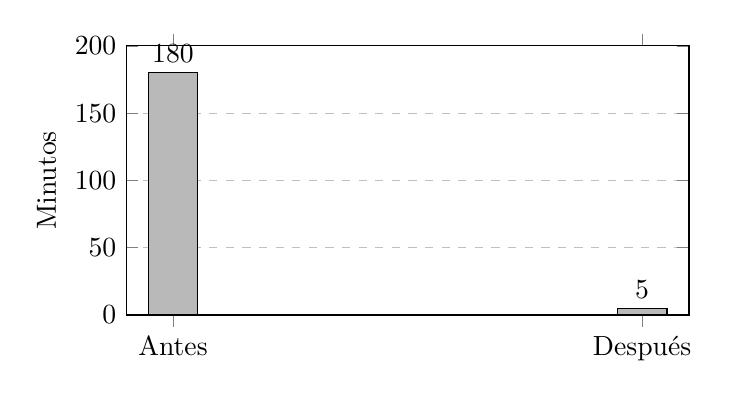
\begin{tikzpicture}
\begin{axis}[ybar,width=0.72\linewidth,height=5cm,bar width=18pt,ymin=0,ymax=200,ylabel={Minutos},symbolic x coords={Antes,Después},xtick=data,nodes near coords,ymajorgrids=true,grid style=dashed]
\addplot[fill=gray!55] coordinates {(Antes,180) (Después,5)};
\end{axis}
\end{tikzpicture}
\end{figure}

\begin{figure}[H]
\centering
\caption{Tasa de errores del módulo de Proveedores antes y después.}\label{fig:cap5_te_proveedores}
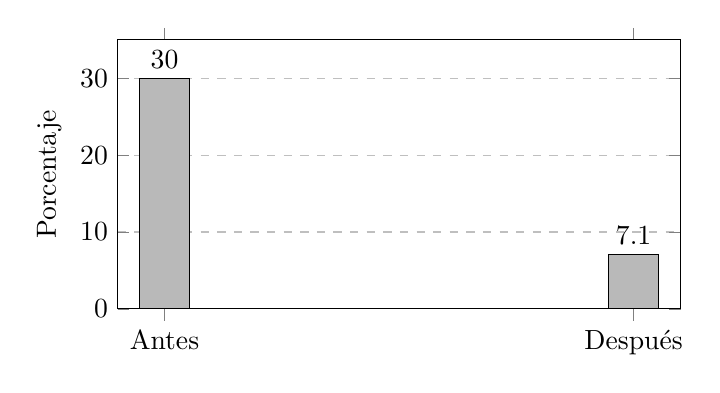
\begin{tikzpicture}
\begin{axis}[ybar,width=0.72\linewidth,height=5cm,bar width=18pt,ymin=0,ymax=35,ylabel={Porcentaje},symbolic x coords={Antes,Después},xtick=data,nodes near coords,ymajorgrids=true,grid style=dashed]
\addplot[fill=gray!55] coordinates {(Antes,30) (Después,7.1)};
\end{axis}
\end{tikzpicture}
\end{figure}

\begin{figure}[H]
\centering
\caption{Personal involucrado en el módulo de Proveedores antes y después.}\label{fig:cap5_personal_proveedores}
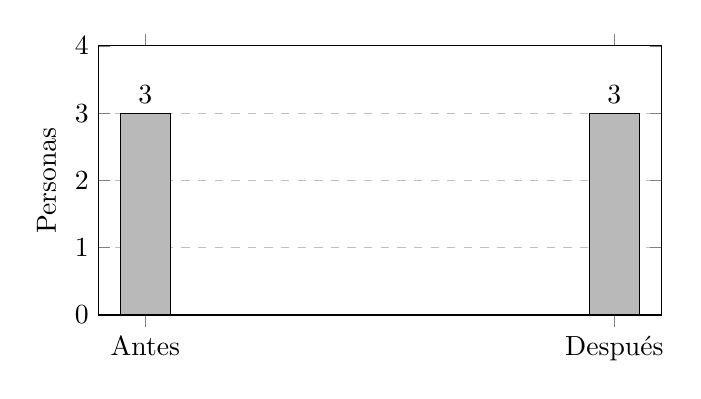
\begin{tikzpicture}
\begin{axis}[ybar,width=0.72\linewidth,height=5cm,bar width=18pt,ymin=0,ymax=4,ylabel={Personas},symbolic x coords={Antes,Después},xtick=data,nodes near coords,ymajorgrids=true,grid style=dashed]
\addplot[fill=gray!55] coordinates {(Antes,3) (Después,3)};
\end{axis}
\end{tikzpicture}
\end{figure}

\begin{figure}[H]
\centering
\caption{Insumos utilizados en el módulo de Proveedores antes y después.}\label{fig:cap5_insumos_proveedores}
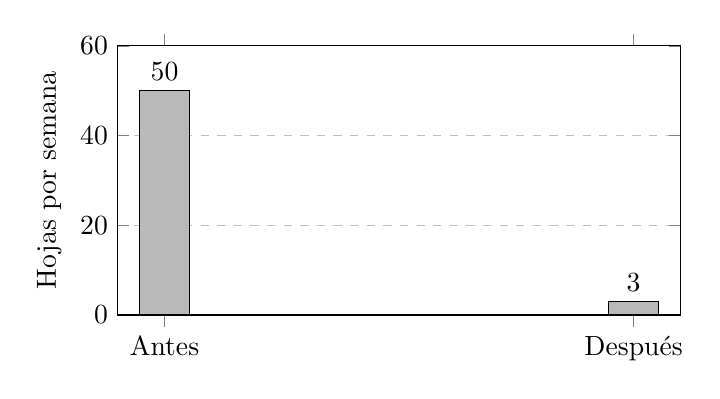
\begin{tikzpicture}
\begin{axis}[ybar,width=0.72\linewidth,height=5cm,bar width=18pt,ymin=0,ymax=60,ylabel={Hojas por semana},symbolic x coords={Antes,Después},xtick=data,nodes near coords,ymajorgrids=true,grid style=dashed]
\addplot[fill=gray!55] coordinates {(Antes,50) (Después,3)};
\end{axis}
\end{tikzpicture}
\end{figure}

\begin{figure}[H]
\centering
\caption{Tiempo de proceso del módulo de Viáticos antes y después.}\label{fig:cap5_tp_viaticos}
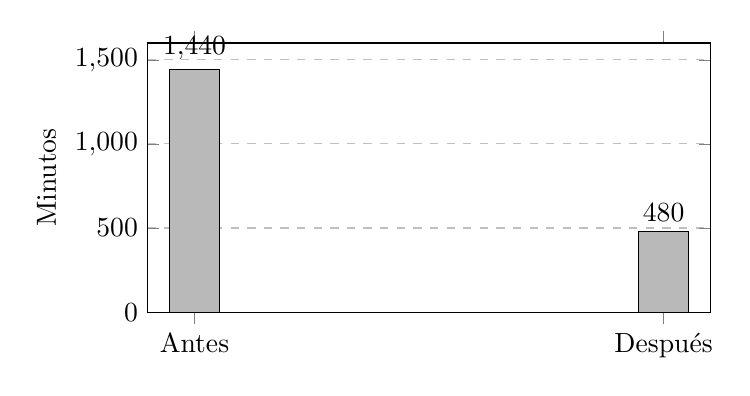
\begin{tikzpicture}
\begin{axis}[ybar,width=0.72\linewidth,height=5cm,bar width=18pt,ymin=0,ymax=1600,ylabel={Minutos},symbolic x coords={Antes,Después},xtick=data,nodes near coords,ymajorgrids=true,grid style=dashed]
\addplot[fill=gray!55] coordinates {(Antes,1440) (Después,480)};
\end{axis}
\end{tikzpicture}
\end{figure}

\begin{figure}[H]
\centering
\caption{Tasa de errores del módulo de Viáticos antes y después.}\label{fig:cap5_te_viaticos}
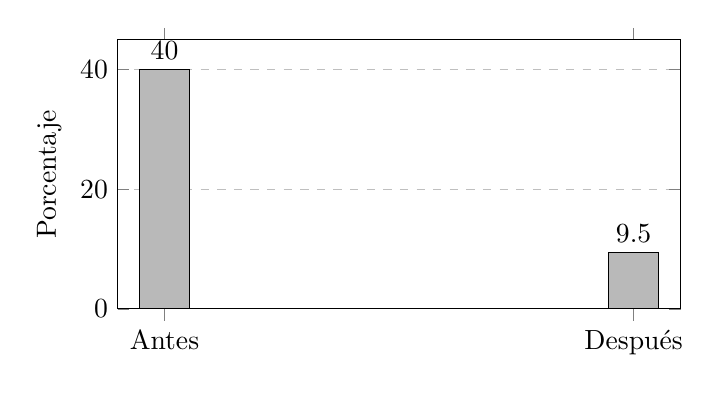
\begin{tikzpicture}
\begin{axis}[ybar,width=0.72\linewidth,height=5cm,bar width=18pt,ymin=0,ymax=45,ylabel={Porcentaje},symbolic x coords={Antes,Después},xtick=data,nodes near coords,ymajorgrids=true,grid style=dashed]
\addplot[fill=gray!55] coordinates {(Antes,40) (Después,9.5)};
\end{axis}
\end{tikzpicture}
\end{figure}

\begin{figure}[H]
\centering
\caption{Personal involucrado en el módulo de Viáticos antes y después.}\label{fig:cap5_personal_viaticos}
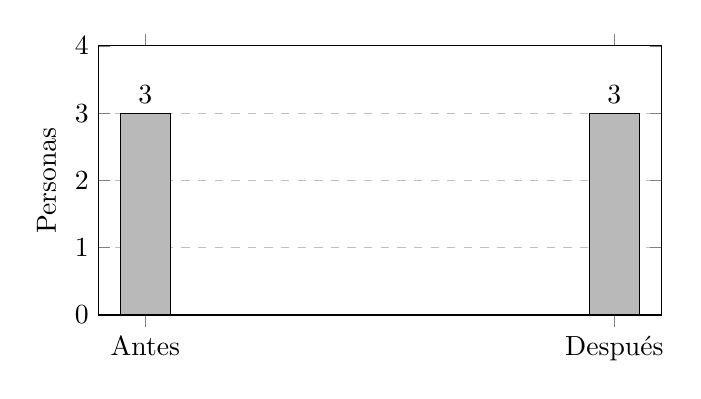
\begin{tikzpicture}
\begin{axis}[ybar,width=0.72\linewidth,height=5cm,bar width=18pt,ymin=0,ymax=4,ylabel={Personas},symbolic x coords={Antes,Después},xtick=data,nodes near coords,ymajorgrids=true,grid style=dashed]
\addplot[fill=gray!55] coordinates {(Antes,3) (Después,3)};
\end{axis}
\end{tikzpicture}
\end{figure}

\begin{figure}[H]
\centering
\caption{Insumos utilizados en el módulo de Viáticos antes y después.}\label{fig:cap5_insumos_viaticos}
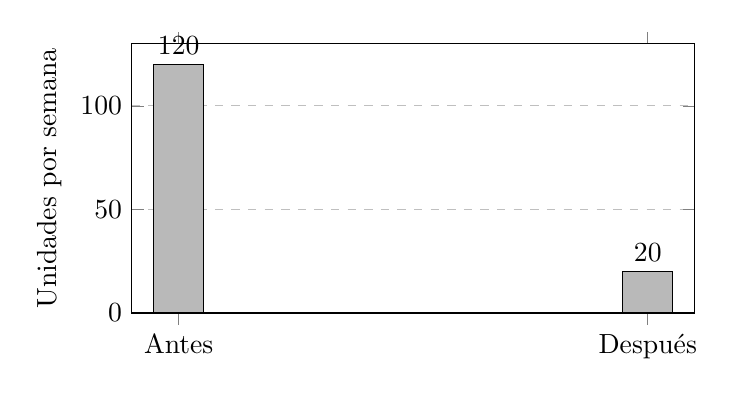
\begin{tikzpicture}
\begin{axis}[ybar,width=0.72\linewidth,height=5cm,bar width=18pt,ymin=0,ymax=130,ylabel={Unidades por semana},symbolic x coords={Antes,Después},xtick=data,nodes near coords,ymajorgrids=true,grid style=dashed]
\addplot[fill=gray!55] coordinates {(Antes,120) (Después,20)};
\end{axis}
\end{tikzpicture}
\end{figure}

\begin{figure}[H]
\centering
\caption{Tiempo de proceso del módulo de Nomenclatura contable antes y después.}\label{fig:cap5_tp_nomenclatura}
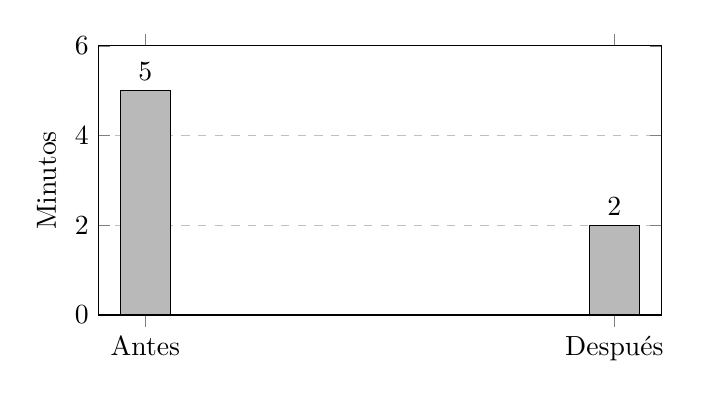
\begin{tikzpicture}
\begin{axis}[ybar,width=0.72\linewidth,height=5cm,bar width=18pt,ymin=0,ymax=6,ylabel={Minutos},symbolic x coords={Antes,Después},xtick=data,nodes near coords,ymajorgrids=true,grid style=dashed]
\addplot[fill=gray!55] coordinates {(Antes,5) (Después,2)};
\end{axis}
\end{tikzpicture}
\end{figure}

\begin{figure}[H]
\centering
\caption{Tasa de errores del módulo de Nomenclatura contable antes y después.}\label{fig:cap5_te_nomenclatura}
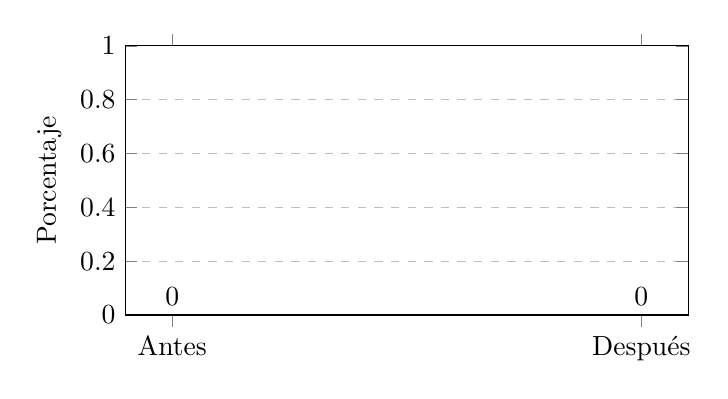
\begin{tikzpicture}
\begin{axis}[ybar,width=0.72\linewidth,height=5cm,bar width=18pt,ymin=0,ymax=1,ylabel={Porcentaje},symbolic x coords={Antes,Después},xtick=data,nodes near coords,ymajorgrids=true,grid style=dashed]
\addplot[fill=gray!55] coordinates {(Antes,0) (Después,0)};
\end{axis}
\end{tikzpicture}
\end{figure}

\begin{figure}[H]
\centering
\caption{Personal involucrado en el módulo de Nomenclatura contable antes y después.}\label{fig:cap5_personal_nomenclatura}
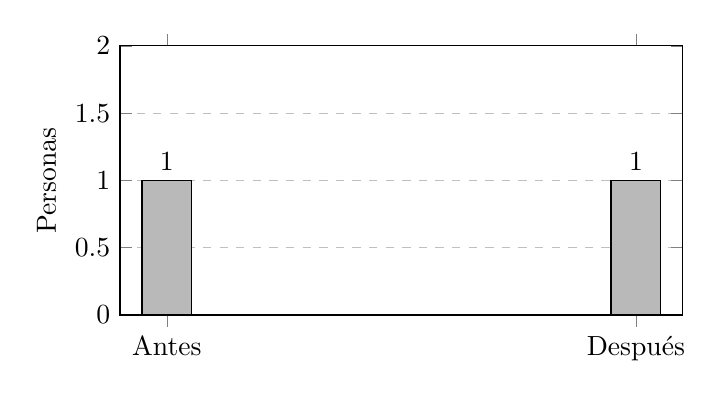
\begin{tikzpicture}
\begin{axis}[ybar,width=0.72\linewidth,height=5cm,bar width=18pt,ymin=0,ymax=2,ylabel={Personas},symbolic x coords={Antes,Después},xtick=data,nodes near coords,ymajorgrids=true,grid style=dashed]
\addplot[fill=gray!55] coordinates {(Antes,1) (Después,1)};
\end{axis}
\end{tikzpicture}
\end{figure}

\begin{figure}[H]
\centering
\caption{Insumos utilizados en el módulo de Nomenclatura contable antes y después.}\label{fig:cap5_insumos_nomenclatura}
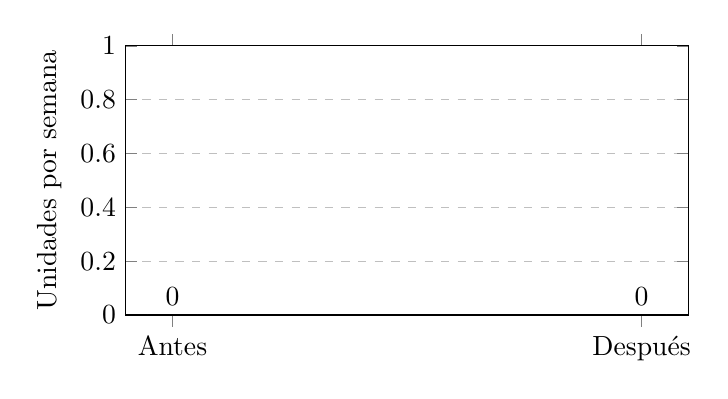
\begin{tikzpicture}
\begin{axis}[ybar,width=0.72\linewidth,height=5cm,bar width=18pt,ymin=0,ymax=1,ylabel={Unidades por semana},symbolic x coords={Antes,Después},xtick=data,nodes near coords,ymajorgrids=true,grid style=dashed]
\addplot[fill=gray!55] coordinates {(Antes,0) (Después,0)};
\end{axis}
\end{tikzpicture}
\end{figure}

\subsection{Flujos de procesos}

La comparación de los flujos permite observar cómo se modificó la secuencia de actividades. Antes de la solución, la información se recibía en documentos separados, se trasladaba entre personas y se consolidaba manualmente. Después, el sistema centraliza los registros, aplica validaciones y genera información disponible para las etapas siguientes.

\subsubsection{Registro y control de proveedores}

Antes de la implementación, el proceso dependía de la consulta de archivos, la verificación manual del NIT y la revisión posterior de la cuenta contable. Después de la implementación, la búsqueda por NIT, la asignación de nomenclatura y la generación de partidas se realizan dentro de un flujo integrado.

\begin{figure}[H]
\centering
\caption{Comparación del flujo de registro y control de proveedores.}\label{fig:cap5_flujo_proveedores}
\begin{tikzpicture}[node distance=0.65cm and 0.35cm, every node/.style={font=\scriptsize, align=center}, box/.style={draw, rounded corners, minimum width=2.2cm, minimum height=0.7cm}, arrow/.style={->, thick}]
\node[box] (a) {Recibir datos y documentos};
\node[box, right=of a] (b) {Revisar archivos manualmente};
\node[box, right=of b] (c) {Validar NIT y cuenta};
\node[box, right=of c] (d) {Registrar y generar partida};
\draw[arrow] (a)--(b)--(c)--(d);
\node[box, below=0.7cm of a] (e) {Buscar proveedor por NIT};
\node[box, right=of e] (f) {Validar datos y retenciones};
\node[box, right=of f] (g) {Asignar cuenta contable};
\node[box, right=of g] (h) {Generar partida y consultar cartera};
\draw[arrow] (e)--(f)--(g)--(h);
\node[left=0.1cm of a, font=\scriptsize\bfseries] {Antes};
\node[left=0.1cm of e, font=\scriptsize\bfseries] {Después};
\end{tikzpicture}
\end{figure}

\subsubsection{Registro y liquidación de viáticos}

El flujo anterior de Viáticos requería recibir liquidaciones, revisar facturas, consultar asignaciones y consolidar los valores antes de generar una partida. El flujo posterior organiza colaboradores, territorios, semanas y categorías, y permite asociar la información de la liquidación con las partidas correspondientes.

\begin{figure}[H]
\centering
\caption{Comparación del flujo de registro y liquidación de viáticos.}\label{fig:cap5_flujo_viaticos}
\begin{tikzpicture}[node distance=0.65cm and 0.35cm, every node/.style={font=\scriptsize, align=center}, box/.style={draw, rounded corners, minimum width=2.2cm, minimum height=0.7cm}, arrow/.style={->, thick}]
\node[box] (a) {Recibir liquidación};
\node[box, right=of a] (b) {Revisar facturas y hojas};
\node[box, right=of b] (c) {Consolidar valores};
\node[box, right=of c] (d) {Preparar partida manual};
\draw[arrow] (a)--(b)--(c)--(d);
\node[box, below=0.7cm of a] (e) {Asignar colaborador, territorio y gira};
\node[box, right=of e] (f) {Clasificar semana y categoría};
\node[box, right=of f] (g) {Asociar facturas y validar};
\node[box, right=of g] (h) {Generar partida semanal};
\draw[arrow] (e)--(f)--(g)--(h);
\node[left=0.1cm of a, font=\scriptsize\bfseries] {Antes};
\node[left=0.1cm of e, font=\scriptsize\bfseries] {Después};
\end{tikzpicture}
\end{figure}

\subsubsection{Clasificación mediante nomenclatura contable}

Antes de la implementación, la cuenta contable se buscaba en listados separados y podía copiarse manualmente en el documento de respaldo. Después de la implementación, el catálogo se consulta desde el sistema y sus cuentas se ofrecen como opciones en los formularios de Proveedores y Viáticos.

\begin{figure}[H]
\centering
\caption{Comparación del flujo de clasificación mediante nomenclatura contable.}\label{fig:cap5_flujo_nomenclatura}
\begin{tikzpicture}[node distance=0.65cm and 0.35cm, every node/.style={font=\scriptsize, align=center}, box/.style={draw, rounded corners, minimum width=2.2cm, minimum height=0.7cm}, arrow/.style={->, thick}]
\node[box] (a) {Recibir concepto del gasto};
\node[box, right=of a] (b) {Buscar en listado separado};
\node[box, right=of b] (c) {Copiar código y nombre};
\node[box, right=of c] (d) {Revisar partida};
\draw[arrow] (a)--(b)--(c)--(d);
\node[box, below=0.7cm of a] (e) {Seleccionar módulo y concepto};
\node[box, right=of e] (f) {Consultar catálogo activo};
\node[box, right=of f] (g) {Seleccionar cuenta Debe/Haber};
\node[box, right=of g] (h) {Usar cuenta en la partida};
\draw[arrow] (e)--(f)--(g)--(h);
\node[left=0.1cm of a, font=\scriptsize\bfseries] {Antes};
\node[left=0.1cm of e, font=\scriptsize\bfseries] {Después};
\end{tikzpicture}
\end{figure}

\subsection{Evaluación resumida de los módulos}

La Tabla~\ref{tab:cap5_resumen} integra los cuatro indicadores solicitados para los tres módulos. La lectura de las diferencias debe considerar que una reducción del TP, la TE o los insumos representa una mejora. En el caso del personal, la ausencia de variación indica que la solución optimizó las actividades sin modificar la cantidad de participantes.

\begin{table}[H]
\centering
\caption{Resumen comparativo de resultados por módulo.}\label{tab:cap5_resumen}
\begingroup
\small
\setlength{\tabcolsep}{4pt}
\begin{tabularx}{0.94\linewidth}{@{}>{\raggedright\arraybackslash}p{2.6cm}>{\raggedright\arraybackslash}X>{\raggedright\arraybackslash}X>{\centering\arraybackslash}p{1.6cm}@{}}
\toprule
\textbf{Módulo} & \textbf{Resultados observados} & \textbf{Causa principal de la mejora} & \textbf{Estado}\\
\midrule
Proveedores & TP: reducción de 97.2\%; TE: reducción de 22.9 pp; insumos: reducción de 47 hojas por semana; personal sin variación. & Consulta por NIT, centralización de datos, selección de cuenta y generación de partidas. & Cumple\\
Viáticos & TP: reducción de 66.7\%; TE: reducción de 30.5 pp; insumos: reducción de 100 unidades por semana; personal sin variación. & Organización de colaboradores, giras, categorías, liquidaciones y partidas semanales. & Cumple\\
Nomenclatura & TP: reducción de 60.0\%; TE, personal e insumos sin variación. & Catálogo centralizado e integración de cuentas con Proveedores y Viáticos. & Cumple\\
\bottomrule
\end{tabularx}
\endgroup
\end{table}

En conjunto, los resultados muestran que el principal efecto del sistema fue reducir el tiempo de ejecución y el uso de insumos. La cantidad de personas se mantuvo constante porque los procesos aún requieren revisión y autorización del personal responsable. La permanencia del personal no contradice la mejora; indica que el sistema funciona como herramienta de apoyo para las personas que ya participan en el proceso.

\subsection{Evaluación de la hipótesis}

La hipótesis de trabajo plantea que la implementación de un sistema complementario de control contable contribuye a mejorar la eficiencia, el control y la precisión en la gestión de documentos contables. Con base en la comparación realizada, la hipótesis se cumple de manera favorable.

En el módulo de Proveedores, el tiempo de proceso disminuyó de 180 a 5 minutos, lo que representa una reducción de 97.2\%. La tasa de errores disminuyó de 30\% a 7.1\%, equivalente a una reducción de 22.9 puntos porcentuales. Además, el consumo de hojas pasó de 50 a 3 por semana. Estos cambios se relacionan con la consulta por NIT, la centralización de la información, la asignación de la cuenta de nomenclatura y la generación integrada de partidas.

En el módulo de Viáticos, el proceso se redujo de tres días laborales a un día laboral, de 1\,440 a 480 minutos, equivalente a una reducción de 66.7\%. La tasa de errores disminuyó de 40\% a 9.5\%, es decir, 30.5 puntos porcentuales. El consumo de insumos se redujo de 120 a 20 unidades por semana. Esta mejora se explica por la organización de colaboradores, territorios, giras, semanas, categorías y liquidaciones en un mismo flujo.

En el módulo de Nomenclatura contable, el tiempo de consulta o registro disminuyó de cinco a dos minutos, equivalente a una reducción de 60.0\%. La tasa de errores operativos permaneció en 0\%, debido a que no se observaron errores en la ejecución normal del proceso. La cantidad de personas y los insumos también permanecieron sin variación. El aporte principal de este módulo fue garantizar que las cuentas estén disponibles desde un catálogo centralizado y puedan reutilizarse en los módulos de Proveedores y Viáticos.

Los resultados funcionales obtenidos complementan este análisis. En las pruebas de Proveedores se aprobaron 26 de 28 casos, en Viáticos 19 de 21 y en Nomenclatura 19 de 21, para un total de 64 aprobados de 70 y un resultado de 91.4\%. La existencia de seis casos que requieren revisión no invalida la hipótesis; por el contrario, muestra que la evaluación permitió identificar aspectos concretos para una etapa posterior de mejora.

En conclusión, la hipótesis se cumple porque el sistema redujo los tiempos de proceso en los tres módulos, disminuyó la tasa de errores en Proveedores y Viáticos, redujo el consumo de insumos y fortaleció la trazabilidad de la información contable. La solución no eliminó la participación del personal, pero sí organizó sus actividades y redujo tareas manuales. Por ello, el sistema Controla constituye una herramienta de apoyo que mejora el control operativo y proporciona una base para continuar optimizando los procesos de la distribuidora farmacéutica.
